% The first command in your LaTeX source must be the \documentclass command.

\documentclass[sigconf]{acmart}
 % Do not change for ICTIR'19

\settopmatter{printacmref=true}
  % mandatory for ICTIR'19

\fancyhead{}
  % do not delete this code.
\usepackage{balance}
  % for creating a balanced last page (usually last page with references)
 %activate todo's
\newcommand{\todo}[1]{\textcolor{red}{TODO: #1}\PackageWarning{TODO:}{#1!}}
% deactivate todos
%\newcommand{\todo}[1]{ \PackageWarning{TODO:}{#1!}}

% defining the \BibTeX command - from Oren Patashnik's original BibTeX documentation.
\def\BibTeX{{\rm B\kern-.05em{\sc i\kern-.025em b}\kern-.08emT\kern-.1667em\lower.7ex\hbox{E}\kern-.125emX}}
    
% Rights management information. 
% This information is sent to you when you complete the rights form.
% These commands have SAMPLE values in them; it is your responsibility as an author to replace
% the commands and values with those provided to you when you complete the rights form.
%
% These commands are for a PROCEEDINGS abstract or paper.

\copyrightyear{2019} 
\acmYear{2019} 
\acmConference[PredictGIS 2019]{ACM SIGSPATIAL Workshop on Prediction of Human Mobility}{November 5, 2019}{Chicago, IL, USA}
\acmBooktitle{The 2019 ACM SIGSPATIAL Workshop on Prediction of Human Mobility (Predict GIS '19), November 5, 2019, Chicago, IL, USA}



% Submission ID. 
% Use this when submitting an article to a sponsored event. You'll receive a unique submission ID from the organizers
% of the event, and this ID should be used as the parameter to this command.
\acmSubmissionID{ictir094s}


% end of the preamble, start of the body of the document source.

\begin{document}

\fancyhead{}
  % do not delete this code.


% The "title" command has an optional parameter, allowing the author to define a "short title" to be used in page headers.
\title{%
  Patterns of Origin Destination Distributions \\
  \large Rules Mining using Massive GPS Trajectory Data}



%
% By default, the full list of authors will be used in the page headers. Often, this list is too long, and will overlap
% other information printed in the page headers. This command allows the author to define a more concise list
% of authors' names for this purpose.
%\renewcommand{\shortauthors}{Chatterjee and Dietz}

%
% The abstract is a short summary of the work to be presented in the article.
\begin{abstract}
Understanding the spatio-temporal distribution of road traffic conditions is imperative to the design of suitable countermeasures for congestion. The amount of crowd sourced data from private aggregators is rapidly expanding to include data sources that were previously not available; this data can assist in developing new approaches and algorithms to understand travel patterns and origin-destination (O-D) distributions. We acquired four months (February, June, July, and October of 2015) of INRIX waypoint data that includes vehicle trips from various sources. To determine the association between demographic, economic, and land use information and O-D patterns, we acquired Census block group level data from American Community Survey (ACS), and block level economic data from Longitudinal Employer-Household Dynamics (LEHD). We provided insights on the relationship between demographic information and O-D patterns by Census spatial unit block group. Based on multi-source data, we used classification-based association rules mining to determine key association patterns. 
\end{abstract}

%
% The code below is generated by the tool at http://dl.acm.org/ccs.cfm.
% Please copy and paste the code instead of the example below.
%
%\begin{CCSXML}
%<ccs2012>
% <concept>
%<concept_id>10002951.10003317.10003338</concept_id>
%<concept_desc>Information systems~Retrieval models and ranking</concept_desc>
%<concept_significance>500</concept_significance>
%</concept>
%</ccs2012>
%<concept>
%<concept_id>10002951.10003317.10003325</concept_id>
%<concept_desc>Information systems~Information retrieval query processing</concept_desc>
%<concept_significance>300</concept_significance>
%</concept>
%\end{CCSXML}
%
%\ccsdesc[500]{Information systems~Retrieval models and ranking}
%\ccsdesc[300]{Information systems~Information retrieval query processing}
%

%
% Keywords. The author(s) should pick words that accurately describe the work being
% presented. Separate the keywords with commas.
% \keywords{joint query-entity-passage features, entity context neighbors, entity salience, entity context document}


%
% This command processes the author and affiliation and title information and builds
% the first part of the formatted document.
\maketitle

\section{Introduction}
\label{sec:Introduction}

Roadside Interview Survey (RSI) has been considered as the common method to determine the measures of roadway origin-destinations (O-D). The crowd sourced data from the private companies can assist in developing new algorithms to understand O-D measures. Although these data sources suffer from many limitations, they are proving valuable insights in determining many traffic operational exposures. Many studies performed analysis on the O-D patterns using different regression models. In general, regression models ignore subgroup or clusters in the data sets. Rules based models can identify the subgroup effects from complex and large data sets without imposing any prior assumptions. 

We acquired four months (February, June, July, and October of 2015) of INRIX waypoint data that includes vehicle trips from various data providers. We provided insights on the relationship between demographic information and O-D patterns. To determine the relationship between O-D patterns and other area specific variables, we acquired Census block group level data from American Community Survey (ACS), and block level economic data from Longitudinal Employer-Household Dynamics (LEHD). We performed our analysis by keeping Census block group as the spatial unit. We applied classification-based association rules mining to determine significant rules.

\section{Literature Review}
\label{sec:related work}
%\paragraph{\textbf{Sentence Retrieval}}
Many recent studies have aimed to determine origin destination patterns using crowd sourced data. Some key studies in this area are briefly described in this section. 

In a study conducted by Sana et al. [1], researchers used information from the Google Aggregated and Anonymized Trips (AAT) to develop a machine learning model and generate the San Francisco Bay Area hourly O-D demand matrices. They found that the developed model could effectively predict dynamic O-D person trip matrices by using both existing and future versions of AAT information. In another study, Ma et al. [2] developed a data-driven structure to estimate daily dynamic O-D. To accomplish this, researchers used high-granular traffic frequency and speed data spanning over many years. The developed framework employed t-Distributed Stochastic Neighbor Embedding (t-SNE) and k-means techniques to statistically cluster regular traffic data into typical traffic models. Fan et al. [3] conducted a study in Guangzhou City, China; they developed an O-D assessment methodology for systematic transit travelers. The researchers used smart card bus transportation data to improve the trip-chain O-D estimation algorithms. The results of the study were useful for the real-world work associated with the O-D estimation. In another study, Ge et al. [4] used aggregated data of mobile phone traces to estimate work-related trips and develop a method to estimate O-D matrices based on maximum entropy principle. The researchers calculated the trip production and attraction by using non-linear programming problem; they then used a matrix fitting problem to distribute trips to each O-D pair. Furthermore, two recent studies used Maryland INRIX waypoint data; one study estimated vehicle miles traveled [5] and another determined the reliability of truck drivers’ routing decisions [6]. 

%\paragraph{\textbf{Entity Relation Explanation}}
 \begin{figure*}
    \centering
    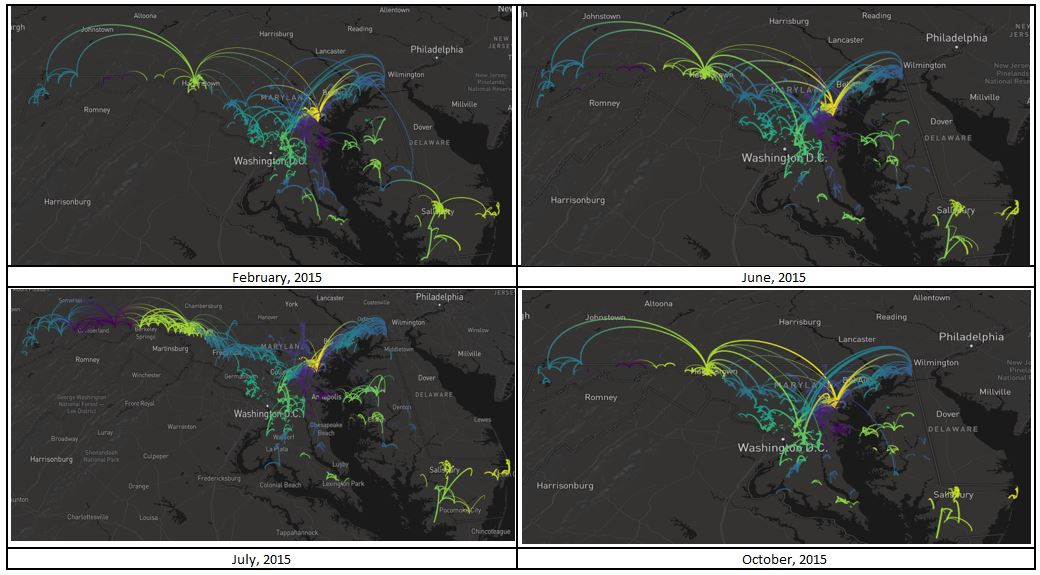
\includegraphics[width=\textwidth]{Fig3a.JPG}
    \caption{O-D patterns by Month}
    \label{fig_dimensions}
 \end{figure*}
 
 
%\paragraph{\textbf{Entity Relation Explanation}}
 \begin{figure*}
    \centering
    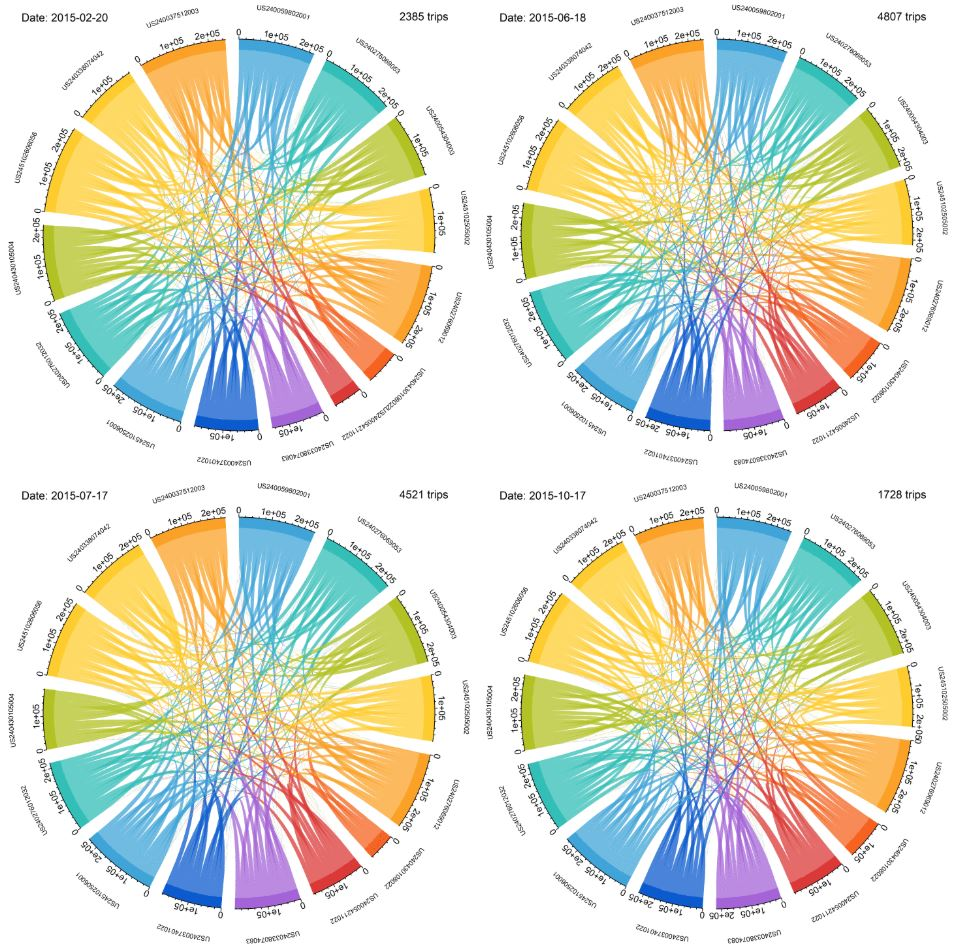
\includegraphics[width=\textwidth]{Fig4.JPG}
    \caption{O-D patterns by Day}
    \label{fig_dimensions}
 \end{figure*}

\section{Approach}
\label{sec:approach}
%  not needed: \subsection{Overview}
%\label{subsec:overview}
\subsection{Data Sources}
\label{subsec:features}
The research team used three separate databases to perform the analysis:
\begin{itemize}
    \item Maryland INRIX waypoint trip data
    \item Census block group level ACS 2013-2017 data
    \item Census block level LEHD 2015 data
\end{itemize}
\subsubsection{Maryland INRIX trip data. }
\label{subsubsec:features:1}
We collected Maryland INRIX trip data to perform the analysis. The acquired data for four months (February, June, July and October 2015) contain three types of monthly files in comma separated value (CSV) format:
\begin{itemize}
    \item TripRecordsReport (trip data)
    \item TripRecordsReportWaypoints (waypoint data)
    \item TripsRecordsReportProviderDetails (information on trip data providers)
\end{itemize}
The acquired data set contains:
\begin{itemize}
    \item 19,690,402 trip information
    \item 1,376,720,203 waypoint (geospatial point recorded by GPS devices that represents the location of the recorded vehicle) information
    \item 5,451,095 unique device identifications
    \item 148 data providers (45 providers)
    \begin{itemize}
        \item 3 providers account for 52 percent of trips
        \item 18 providers account for 99 percent of trips
    \end{itemize}    
    \item Four types of vehicle driving profiles: 1) consumer vehicles, 2) taxi/shuttle/town car service fleets, 3) local delivery fleets, and 4) for-hire/private trucking fleets.
    \item Three vehicle weight classes: 1) light duty truck/passenger vehicle (0 to 14000 lbs.), 2) medium duty truck/vans (14001 to 26000 lbs.), and 3) heavy-duty truck (greater than 26000 lbs.).
\end{itemize}


\subsubsection{ACS Data}
\label{subsubsec:feature:2}
The ACS data, acquired from the U.S. Census Bureau's Decennial Census Program, provide details of demographic, social, housing, and economic estimates for different spatial area units including Census tract, and block groups. We used ACS five-year (2013-2017) estimates for Maryland. The research team collected a wider list of variables in the preliminary analysis.  

\subsubsection{LEHD Data. }
\label{subsubsec:feature:3}
We also used the Census block data of LEHD Origin-Destination Employment Statistics (LODES) 2015 data. The LODES files contain data for Residential Area Characteristics (RAC) and Work Area Characteristics (WAC). 

\subsection{Data Integration}
\label{subsec:features}
The data integration steps
\begin{itemize}
    \item The collected ACS data contains different tables such as age, gender, income, and household. We selected key demographic and relevant information for this analysis. 
    \item  The block level RAC and WAC data were merged into block group level. 
    \item We used QGIS tool to spatially merge origin and destination data with census block groups level information. Later several separate databases were developed based on the following:
    \begin{itemize}
        \item Monthly O-D data by block groups
        \item Daily O-D data by block groups    
        \item Hourly O-D data by block groups
        \item O-D data by vehicle types  
    \end{itemize}
\end{itemize}

%\paragraph{\textbf{Entity Relation Explanation}}
\begin{figure}
    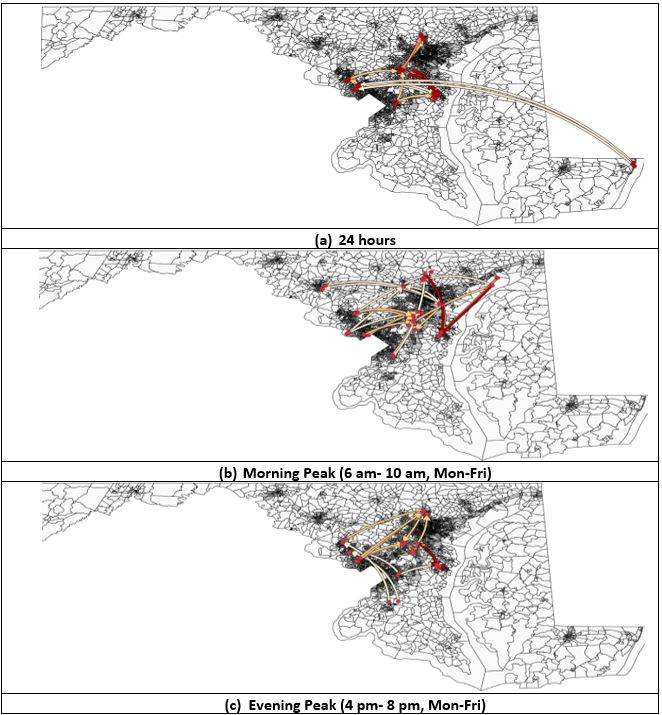
\includegraphics[width=\columnwidth]{Fig2a.JPG}
    \caption{Hourly O-D patterns by consumer vehicles}
    \label{fig_dimensions}
\end{figure}

%\paragraph{\textbf{Entity Relation Explanation}}
\begin{figure}
    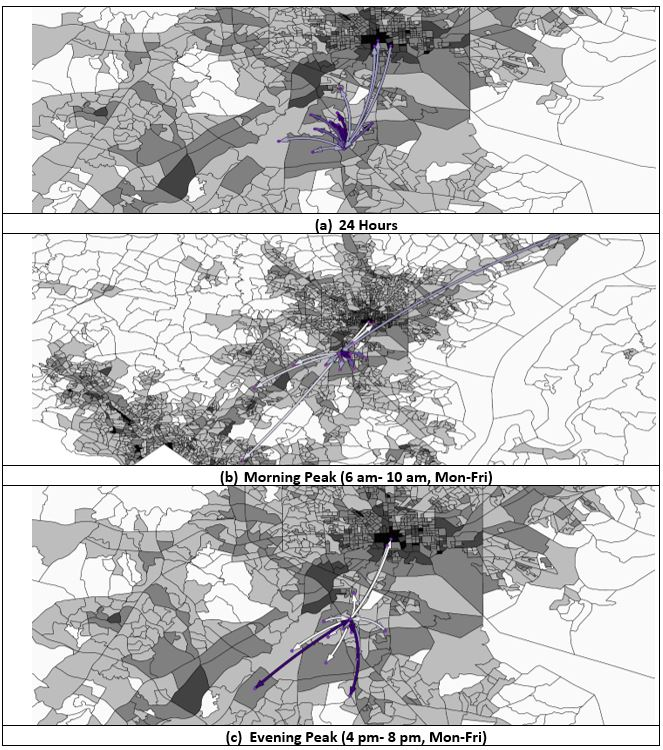
\includegraphics[width=\columnwidth]{Fig1a.JPG}
    \caption{Hourly O-D patterns by taxi and shuttles}
    \label{fig_dimensions}
\end{figure}
 

\section{Evaluation}
\label{sec:Evaluation}
\subsection{Research Questions}
\label{subsec:research questions}
We developed several key research questions:
\begin{itemize}
\item[\textbf{RQ1}] How do O-D patterns differ by different temporal units (for example, hour, month, day of the week) and vehicle types?
\item[\textbf{RQ2}] How can we improve the conventional O-D visualizations? 
\item[\textbf{RQ3}] What are key contributors for different O-D patterns?
\end{itemize}

\subsection{O-D Distribution}
\label{subsec:Evaluation Paradigm}
It is important to determine the key O-D matrices for different scenarios. Three different temporal patterns were used for analysis: 1) all 24 hours, 2) morning peak (6-10 am, Mon-Fri), and 3) evening peak (4-8 pm, Mon-Fri). Figure 2 indicates that the top O-D generators vary by different temporal slices. 

To answer RQ1 and RQ2, we developed several different data visualization tools to provide additional insights on the data. Figure 1 illustrates the O-D patterns by month. The color of the nodes are based on the distances. The overall trends look similar for three months (February, June, and October). However, the patterns of July is significantly different from the other three months.  

A chord diagram, resourceful in comparing the similarities and patterns within a dataset, illustrates the interrelationships between individuals (for this study, each block group is considered as individual spatial unit). The associations between individual block groups are used in displaying commonality of information or interest. Nodes are arranged in a circular form, with the association between points connected to each other either with arcs or curves. The assigned values to each of the connection are represented proportionally by the size of each arc. The color is used in grouping the data into different categories that aid in making comparisons and distinguishing groups. Figure 2, the static version of the interactive chord diagram tool, indicates that the in-betweenness between the O-D pairs is significant. An interactive version will provide 

Figure 3 and Figure 4 show the top 20 O-D pairs for two consumer vehicles, and taxis/shuttles respectively. The O-D patterns of the consumer vehicles show higher distances between the origin and destinations. Taxi or shuttle trips are rather short and mostly in between the major urban locations. The top O-D pairs also differ by different temporal clusters for both consumer vehicle trips and taxis/shuttles.  

\section{Results}
\label{subsubsec: reults}
\subsection{Rules Mining}
\label{subsec:Rules Mining}
We used classification-based association rules to develop the rules associated with O-D patterns. The association rule can be represented as $Antecedent (A) \rightarrow Consequent (B)$, where both

of them are disjoint itemsets. Here, $Support\ of\ antecedent,\ S\left(A\right)=\frac{\sigma(A)}{N};\ Support\ of\ consequent,\ S\left(B\right)=\frac{\sigma(B)}{N};$ and Support of the rule  can be written as 
$Suppport\ of\ rule\ or\ S\left(A\rightarrow B\right)=\frac{\sigma(A\cap B)}{N};$
The measure of reliability for a generated rule is known as confidence ($C\left(A\rightarrow B\right)=\frac{S\left(A\rightarrow B\right)}{S(A)}$).  

The lift ($L\left(A\rightarrow B\right)=\frac{S\left(A\rightarrow B\right)}{S\left(A\right).S(B)}$) is a measure that represents the ratio of confidence and expected confidence. A lift value greater than one shows positive interdependence between A and B, while a value smaller than one refers negative interdependence, and a value of one signifies independence.

We selected the significant variables by performing random forest algorithm. The selected variables (block group level) for model development include average O-D measure, total population (Popu), households (HH), households with family (HH\_F), total WAC jobs (Total\_Jobs\_WAC), and household median income (HH\_MedInc). The top 40 rules with high lift values are listed in Table 1. Average O-D measures per block group are divided into five classes based on the quantile percentages: TQ= 1 [1-20 percent], TQ= 2 [21-40 percent], TQ= 3 [41-60 percent], TQ= 4 [61-80 percent], and TQ=5 [81-100 percent]. For example, TQ=5 indicates the block groups with top 20 percent percent of the O-D trips. The findings show that higher number of populations, WAC, and households are associated with higher   number of O-D trips. The rules provide several breakpoints of the variable clusters to determine the top rules. 	

\begin{table*}[t]
  \centering
  \caption{Top 40 Rules.}
  \label{tab:results}
\begin{tabular}{|l|l|l|l|l|l|}
\hline
Antece.                                                                                & Conse. & S    & C    & L    & Counts \\ \hline
Total\_Jobs\_WAC=(\textgreater 3778.5{]}, HH\_F=(386.5; 659.5{]}                       & TQ=5   & 0.01 & 1    & 5    & 35     \\ \hline
Total\_Jobs\_WAC=(\textgreater 3778.5{]}, Popu=(1366.5; 1978.5{]}                      & TQ=5   & 0.01 & 1    & 5    & 34     \\ \hline
Total\_Jobs\_WAC=(\textgreater 3778.5{]}, Popu=(1978.5; 3311.5{]}                      & TQ=5   & 0.01 & 1    & 5    & 31     \\ \hline
Total\_Jobs\_WAC=(\textgreater 3778.5{]}, HH\_MedInc=(\textgreater 98467{]}            & TQ=5   & 0.01 & 1    & 5    & 28     \\ \hline
Total\_Jobs\_WAC=(\textgreater 3778.5{]}, HH\_MedInc=(53774; 98467{]}                  & TQ=5   & 0.02 & 0.98 & 4.92 & 61     \\ \hline
Total\_Jobs\_WAC=(\textgreater 3778.5{]}                                               & TQ=5   & 0.03 & 0.96 & 4.82 & 109    \\ \hline
Popu=(\textgreater 3311.5{]}, HH=(\textgreater 1252.5{]}, HH\_F=(\textgreater 934.5{]} & TQ=5   & 0.01 & 0.91 & 4.53 & 29     \\ \hline
Total\_Jobs\_WAC={[}\textless 21.5{]}, HH={[}\textless 264.5{]}                        & TQ=1   & 0.02 & 0.9  & 4.52 & 75     \\ \hline
Total\_Jobs\_WAC={[}\textless 21.5{]}, HH\_F={[}\textless 230.5{]}                     & TQ=1   & 0.04 & 0.88 & 4.41 & 157    \\ \hline
Total\_Jobs\_WAC=(833; 3778.5{]}, HH=(\textgreater 1252.5{]}                           & TQ=5   & 0.01 & 0.88 & 4.4  & 22     \\ \hline
HH=(\textgreater 1252.5{]}, HH\_MedInc=(\textgreater 98467{]}                          & TQ=5   & 0.01 & 0.88 & 4.38 & 21     \\ \hline
Total\_Jobs\_WAC={[}\textless 21.5{]}, HH\_MedInc={[}\textless 53774{]}                & TQ=1   & 0.04 & 0.82 & 4.08 & 137    \\ \hline
Popu=(\textgreater 3311.5{]}, HH\_F=(\textgreater 934.5{]}                             & TQ=5   & 0.01 & 0.81 & 4.05 & 34     \\ \hline
Total\_Jobs\_WAC={[}\textless 21.5{]}, Popu=(623.5; 1366.5{]}                          & TQ=1   & 0.05 & 0.81 & 4.03 & 171    \\ \hline
Total\_Jobs\_WAC=(833; 3778.5{]}, HH\_F=(659.5; 934.5{]}                               & TQ=5   & 0.01 & 0.8  & 4    & 52     \\ \hline
Total\_Jobs\_WAC={[}\textless 21.5{]}, HH=(264.5; 477.5{]}                             & TQ=1   & 0.04 & 0.8  & 3.99 & 155    \\ \hline
Total\_Jobs\_WAC=(833; 3778.5{]}, HH=(972.5; 1252.5{]}                                 & TQ=5   & 0.02 & 0.79 & 3.97 & 58     \\ \hline
Popu=(\textgreater 3311.5{]}, HH=(\textgreater 1252.5{]}                               & TQ=5   & 0.01 & 0.79 & 3.95 & 45     \\ \hline
Total\_Jobs\_WAC=(21.5; 61.5{]}, Popu={[}\textless 623.5{]}                            & TQ=1   & 0.01 & 0.78 & 3.91 & 36     \\ \hline
Total\_Jobs\_WAC=(833; 3778.5{]}, HH\_MedInc=(\textgreater 98467{]}                    & TQ=5   & 0.03 & 0.78 & 3.89 & 102    \\ \hline
Total\_Jobs\_WAC=(61.5; 120.5{]}, Popu={[}\textless 623.5{]}                           & TQ=1   & 0.01 & 0.78 & 3.89 & 28     \\ \hline
Total\_Jobs\_WAC=(833; 3778.5{]}, Popu=(\textgreater 3311.5{]}                         & TQ=5   & 0.01 & 0.76 & 3.82 & 26     \\ \hline
HH\_F=(\textgreater 934.5{]}                                                           & TQ=5   & 0.01 & 0.76 & 3.8  & 35     \\ \hline
Total\_Jobs\_WAC=(833; 3778.5{]}, Popu=(1978.5; 3311.5{]}                              & TQ=5   & 0.03 & 0.76 & 3.8  & 123    \\ \hline
Total\_Jobs\_WAC=(833; 3778.5{]}, HH\_F=(386.5; 659.5{]}                               & TQ=5   & 0.04 & 0.75 & 3.77 & 141    \\ \hline
Popu=(\textgreater 3311.5{]}, HH\_MedInc=(\textgreater 98467{]}                        & TQ=5   & 0.01 & 0.73 & 3.66 & 30     \\ \hline
HH=(\textgreater 1252.5{]}                                                             & TQ=5   & 0.02 & 0.72 & 3.59 & 61     \\ \hline
Total\_Jobs\_WAC={[}\textless 21.5{]}                                                  & TQ=1   & 0.07 & 0.72 & 3.58 & 275    \\ \hline
Total\_Jobs\_WAC=(833; 3778.5{]}, HH\_MedInc=(53774; 98467{]}                          & TQ=5   & 0.05 & 0.71 & 3.55 & 179    \\ \hline
Total\_Jobs\_WAC=(833; 3778.5{]}, HH=(609.5; 972.5{]}                                  & TQ=5   & 0.03 & 0.71 & 3.54 & 131    \\ \hline
Total\_Jobs\_WAC=(21.5; 61.5{]}, HH={[}\textless 264.5{]}                              & TQ=1   & 0.01 & 0.71 & 3.54 & 46     \\ \hline
Total\_Jobs\_WAC=(833; 3778.5{]}, Popu=(1366.5; 1978.5{]}                              & TQ=5   & 0.03 & 0.71 & 3.54 & 99     \\ \hline
Total\_Jobs\_WAC=(833; 3778.5{]}                                                       & TQ=5   & 0.1  & 0.69 & 3.45 & 362    \\ \hline
Total\_Jobs\_WAC=(61.5; 120.5{]}, HH={[}\textless 264.5{]}                             & TQ=1   & 0.01 & 0.67 & 3.33 & 30     \\ \hline
Popu={[}\textless 623.5{]}, HH\_MedInc={[}\textless 53774{]}                           & TQ=1   & 0.02 & 0.66 & 3.31 & 94     \\ \hline
Total\_Jobs\_WAC=(21.5; 61.5{]}, HH\_F={[}\textless 230.5{]}                           & TQ=1   & 0.02 & 0.64 & 3.18 & 89     \\ \hline
Popu={[}\textless 623.5{]}, HH={[}\textless 264.5{]}                                   & TQ=1   & 0.03 & 0.62 & 3.08 & 122    \\ \hline
HH={[}\textless 264.5{]}, HH\_MedInc={[}\textless 53774{]}                             & TQ=1   & 0.03 & 0.6  & 3.01 & 98     \\ \hline
Total\_Jobs\_WAC=(405.5; 833{]}, HH=(972.5; 1252.5{]}                                  & TQ=4   & 0.01 & 0.58 & 2.91 & 25     \\ \hline
HH=(972.5; 1252.5{]}, HH\_MedInc=(\textgreater 98467{]}                                & TQ=5   & 0.01 & 0.56 & 2.81 & 32     \\ \hline
\end{tabular}
\end{table*}

Below, we discuss each of the research questions presented in Section \ref{subsec:research questions}.

\textbf{RQ1:} We observe in Figure 1 that majority of the monthly O-D patterns are similar. The daily O-D patterns by the top 20 O-D generators indicate that range of daily trips in the block groups differ in values to some extent.The trip distribution by vehicle types also differ in patterns. The top consumer vehicle O-D generators have distance measures than the top O-D generators for taxis/shuttles. 


\textbf{RQ2:} Data visualization is an integral part of data-driven analysis. A carefully developed data visualization delivers a powerful cognitive advantage to its viewers. We aimed to develop well-designed and interactive visualization to provide the end users a spontaneous and reactive impression and help them to cut through the clutter of complex data dynamics. We used different data visualization libraries such as D3.js and deck.gl to developed O-D visualizations with important matrices. We have opensourced the codes developed for this study in Github. 

\textbf{RQ3:} We observe that rules mining provided top 40 association rules that do not need any kind of prior assumptions. As earlier studies did not explore rules mining on O-D data sets, the findings from this study can shed some lights in this unexplored research domain. The current analysis is limited to only 40 top rules. However, more insightful rules can be developed by using different thresholds of support and confidence. 

\section{Conclusion and Future Work}
\label{sec: conclusion}
The current study framework was applied to 19.8 million raw GPS vehicle trajectories collected in 2015 in Maryland. The results showed that distribution of O-D measures for different vehicle types vary by hour and by month. The top 20 block groups with high average O-D measure contribute approximately 8.5 percent of trips. The generated top 40 rules provide several breakpoints of the key variables for appropriate rule development. The generated rules can be used for developing appropriate strategies in a way to improve the travel experiences of the roadway users.

The current study is not without limitation. The rules mining applied in this study is limited to monthly O-D data. Future studies should explore the rules with more granular levels of data (for example, daily or hourly). Additionally, the current study is limited to only four months of data from 2015. A more comprehensive data is required to develop a robust framework of O-D measures. 


\bibliographystyle{ACM-Reference-Format}
\bibliography{bibliography}
\begin{enumerate}
\item Sana, B., J. Castiglione, D. Cooper, and D. Tischler. Using Google Passive Data and Machine Learning for Origin-Destination Demand Estimation. Transportation Research Record, Vol 2672, Issue 46, 2018, p. pp 73\textemdash82.
\item  Ma, W., and Z. Qian. Estimating Multi-Year 24/7 Origin-Destination Demand Using High-Granular Multi-Source Traffic Data. Transportation Research Part C: Emerging Technologies, Vol. 96, 2018, pp. 96\textemdash121. 
\item Fan., W, and Z. Chen. Estimation of origin-destination matrix and identification of user activities using public transit smart card data. Center for Advanced Multimodal Mobility Solutions and Education, 2018. 
\item Ge, Q., and F. Daisuke. Updating Origin–Destination Matrices with Aggregated Data of GPS Traces. Transportation Research Part C: Emerging Technologies, Vol. 69, 2016, pp. 291\textemdash312.
\item Fan, J., C. Fu, K. Stewart, and L. Zhang. Using big GPS trajectory data analytics for vehicle miles traveled estimation. Transportation Research Part C, Vol. 103, 2019, pp. 298 \textemdash 307. 
\item Kong, X., W. Eisele, Y. Zhang, and D. Cline. Evaluating the Impact of Real-time Mobility and Travel Time Reliability Information on Truck Drivers’ Routing Decisions. Transportation Research Record: Journal of the Transportation Research Board. Vol. 2672, 2018, pp. 164\textemdash172.
\end{enumerate}
\end{enumerate}




\end{document}
